\newpage
\section{FaaS (Function as a Service)}

\subsection{AWS Lambda}
FaaS è nato con AWS Lambda, che permette agli utenti di mandare in esecuzione del codice (funzione in Lambda) senza gestire i server.\\
L’utente carica il codice sulla piattaforma e Lambda esegue il codice e scala opportunamente. Quindi l’utente non si preoccupa nemmeno dell’esistenza delle macchine virtuali o meccanismi di virtualizzazione.\\
Un’altra funzionalità è quella di associare automaticamente al codice dei \textbf{trigger}, ovvero degli eventi che triggerano l’esecuzione della funzione. Ci sono tre modi per mandare in esecuzione la funzione:
\begin{enumerate}
    \item Caricare una funzione che l'utente ha già definito
    \item Usare l'IDE di AWS per scrivere la funzione
    \item Scegliere tra uno dei template forniti di Lambda
\end{enumerate}

Una volta passata la funzione, Lambda la manda in esecuzione automaticamente ad ogni risveglio del trigger e si preoccupa di tutta la gestione dell’infrastruttura: scalabilità, amministrazione, fornendo anche metriche e logs.\\
Tutto questo ad un costo di servizio calcolato in base alla \textbf{durata} dell’esecuzione della funzione e alla \textbf{memoria} utilizzata.

\paragraph{Prezzi} Amazon fa pagare \$0.20/milione di richieste che riceve la funzione e \$0.0000166667 per ogni GB/s\\
\textit{Esempio}: si assume che un utente alloca 512MB di memoria per la funzione che viene usata 3 milioni di volte in un mese con un durata di 1 secondo ogni volta.\\
Costo delle richieste: $$\frac{3,000,000}{1,000,000} \cdot \$0.20 = \$0.60$$ + Costo della durata: $$ (3,000,000 \cdot 1) * \frac{512}{1024} \cdot \$0.0000166667 = \$25 $$
= \$25.60 totale
 
Anche AWS Lambda è un modello Freemium, infatti esiste il piano free con 1 milione di richieste e 400,000 GB/s di compute time al mese, quindi riconsiderando l'esempio precedente:\\
Costo per le richieste: $$\frac{3,000,000 - 1,000,000}{1,000,000} \cdot \$0.20 = \$0.40$$
Costo per la durata: $$ (3,000,000 \cdot ( \frac{512}{1024} ) - 400,000) \cdot \$0.0000166667 = \$18.33 $$
= \$18.73 totale

\paragraph{Youtube}
\begin{itemize}
    \item \href{https://www.youtube.com/watch?v=eOBq__h4OJ4}{Introduzione AWS Lambda}
    \item \href{https://www.youtube.com/watch?v=PEatXsXIkLc}{Lambda function in Node}
    \item \href{https://www.youtube.com/watch?v=DSrg7hG-jV4}{Connecting Lambda to API Gateway}
\end{itemize}

\subsection{Quale FaaS usare?}
Uno studio ha comparato 10 tra loro 10 diverse piattaforme FaaS basandosi su Business view e Technical view: la conclusione non c'è una piattaforma migliore, dipende da quali sono i bisogni dell’azienda o di chi sviluppa l’app.\\
\textit{FaaStener Prototype} permette di scegliere il FaaS più adatto in base alle proprie necessità. Il fatto di poter scrivere così facilmente le funzioni e renderle collegabili è un grosso vantaggio in termini di velocità di sviluppo e velocizza anche la fase di testing. 
Di contro una volta sviluppata tutta l’applicazione, se si vuole cambiare provider bisogna modificare il codice sorgente. Ci sono comunque delle strategie per uscire o quantomeno ridurre il lock-in, ma se non si vuole rischiare si può sempre scegliere di usare l’open source

\newpage
\begin{figure}[h!]
    \centering
    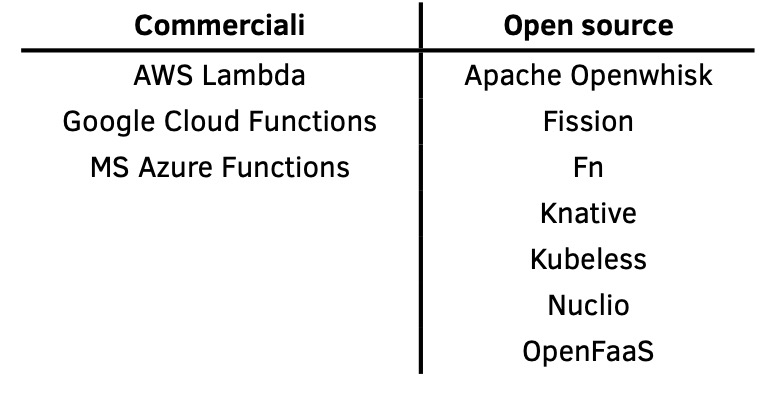
\includegraphics[width=0.5\textwidth]{13.png}
    \caption{FaaS commerciali vs Open Source}
    %\label{fig:enter-label}
\end{figure}

\paragraph{Business view}
\begin{itemize}
    \item Licensing: tutte le FaaS commerciali usano licenze proprietarie, a parte Azure che usa alcune open source. Tutte le FaaS open source usano Apache 2.0, quindi una licenza permissiva
    \item Installation: i server FaaS possono essere usati \textit{on-premise}, ovvero attraverso l’installazione, oppure \textit{as-a-service}, ovvero l’utilizzo del FaaS come servizio. Quasi tutte quelle open source sono disponibili on-premise mentre quelle commerciali sono as-a-service, tranne Azure che può essere installato
    \item Source code: le piattaforme commerciali non sono rilasciate come open source (ad eccezione di alcune parti di Azure). La scelta di un FaaS open source riduce i problemi di vendor lock-in
    \item Release: tutte le piattaforme commerciali sono sempre aggiornate e in produzione, mentre gli open source sono leggermente indietro rispetto alle piattaforme commerciali
    \item Interface: come l’operatore interagisce con il FaaS. Tutte le piattaforme supportano CLI, mentre API e le GUI non sono sempre fornite
    \item Community: GitHub è quello più utilizzato per gli open source. Su Stack Overflow c'è quasi tutto su AWS Lambda
    \item Documentation: tutte le piattaforme forniscono la documentazione su come sviluppare applicazioni e su come possiamo utilizzare la piattaforma. Per quanto riguarda lo sviluppo della piattaforma e dell’architettura, le piattaforme open source non forniscono molti dettagli
\end{itemize}


\paragraph{Technical view}
\begin{itemize}
    \item Development: i linguaggi di programmazione più supportati sono Java, Node.js, Python. Docker è sempre più supportato per poter personalizzare il runtime. La possibilità di usare degli editor o IDE è offerta dalla piattaforme commerciali
    \item Versioning: nel ciclo di vita di un progetto software ci sono più versioni della stessa applicazione. Questo è un punto di debolezza per le open source perché permettono spesso di fare solo implicit version. Le piattaforme commerciali permettono invece di avere dei meccanismi dedicati
    \item Event sources: tutte le piattaforme supportano l’invocazione sincrona basata su HTTP, mentre le invocazioni asincrone sono supportate da poche piattaforme. Molte piattaforme utilizzano schedulers per gestire il flusso di dati
    \item Function orchestration: nel codice ci possono essere più funzioni combinate tra loro. La maggioranza delle piattaforme offre un ”orchestratore” di funzioni dedicato, la metà delle piattaforme usano dei DSL specifici per i workflow, diagrammi di flusso, ...
    \item Testing e debugging: quasi tutte le piattaforme permettono di fare sia testing che debugging. Nelle piattaforme commerciali il testing e debugging sono integrate all’interno dell’ambiente. Nelle piattaforme open source si possono fare solo dei test call o debugging basato sui log
    \item Observability: per monitorare l’applicazione, gli strumenti sono forniti dal provider stesso in caso di piattaforme commerciali, mentre gli open source integrano servizi di terze parti.
    \item Application delivery: quasi tutte le piattaforme usano un approccio dichiarativo al deployment, cioè permettono all’utente di dichiarare qual è lo stato che vuole raggiungere, senza dover dichiarare i passi per raggiungerlo
    \item Code re-use: Lambda e Azure offrono tante funzioni built-in
    \item Access Management: per la gestione degli accessi, le piattaforme commerciali supportano autenticazione alle risorse mentre gli open source si appoggiano a servizi esterni
\end{itemize}